\section{Modelo Completo}
\label{sec:non_arx}
%===============================================================================

Como apresentado na sec�o (\ref{sec:arx}) o modelo ARX n�o consegue representar o
sistema (\ref{eq:system}) completamente, e a estimativa dos parametros da Func�o
de transferencia s�o polarizados. Para contornar este problema utilizaremos um
modelo para descrever o sistema (\ref{eq:system}) de forma completa.

O modelo escolhido para representar o sistema real � apresentado em (\ref{eq:compl}).

\begin{equation}
G(q, \theta )=\frac{a}{q-b}\;\;\;\;\;H(q, \theta)=\frac{q-c}{q-d}
\label{eq:compl}
\end{equation}

utilizando o estimador �timo (\ref{eq:estimador}) obtem-se a equac�o de diferencas apresentada
em (\ref{eq:gmq_eq}). Utilizando o script \ref{anx_gmq_simul} obtem-se o resultado para os parametros
$a$, $b$, $c$ e $d$ para a func�o $G(q, \theta)$ e $H(q, \theta)$.

%\begin{equation}
%\hat{y}(t/t-1, \theta)=H^{-1}(q, \theta)G(q, \theta)u(t)+\[1-H^{-1}(q, \theta)\]y(t)
%\label{eq:estimador}
%\end{equation}

\begin{equation}
\hat{y}(t/t-1, \theta)=a\;u(t-1)-ad\;u(t-2)+(d-c)y(t-1)\\
-b(d-c)y(t-2)+(b+c)\hat{y}(t-1/t-2, \theta)-cb\;\hat{y}(t-2/t-3, \theta)
\label{eq:estimador}
\end{equation}

\begin{figure}[htbp]
	\center
	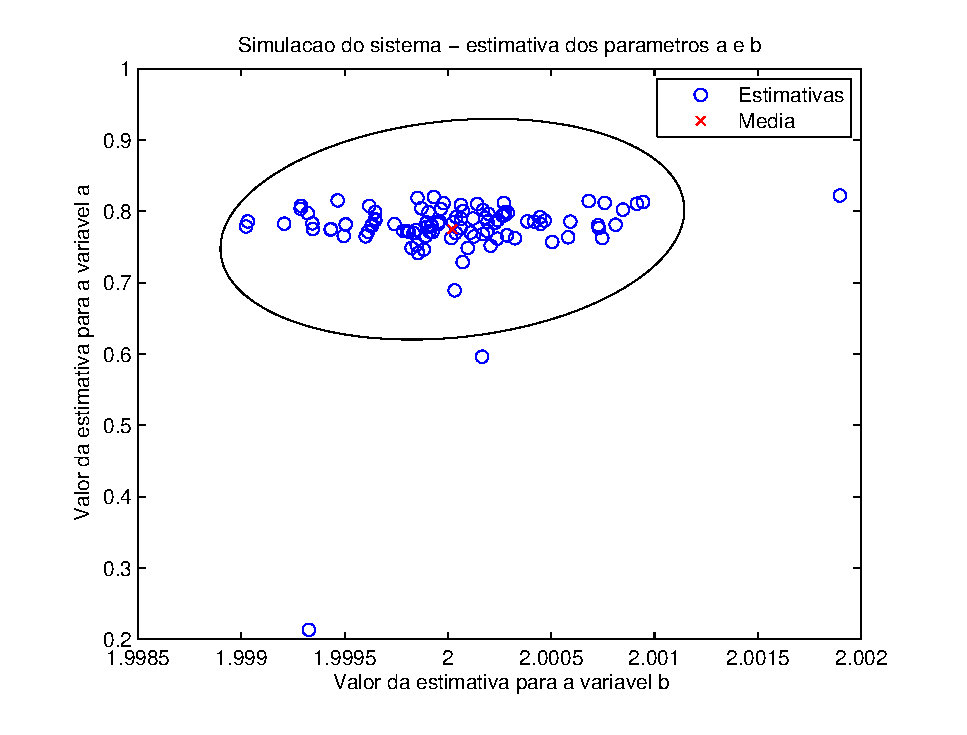
\includegraphics[width=0.98\columnwidth]{figures/gmq_ab.eps}
	\caption{Simulac�o do sistema para uma entrada aleat�ria e utilizando o modelo completo - 
		variaveis do processo $G(q)$ $a$ e $b$.}
	\label{fig:gmq_ab}
\end{figure}

\begin{figure}[htbp]
	\center
	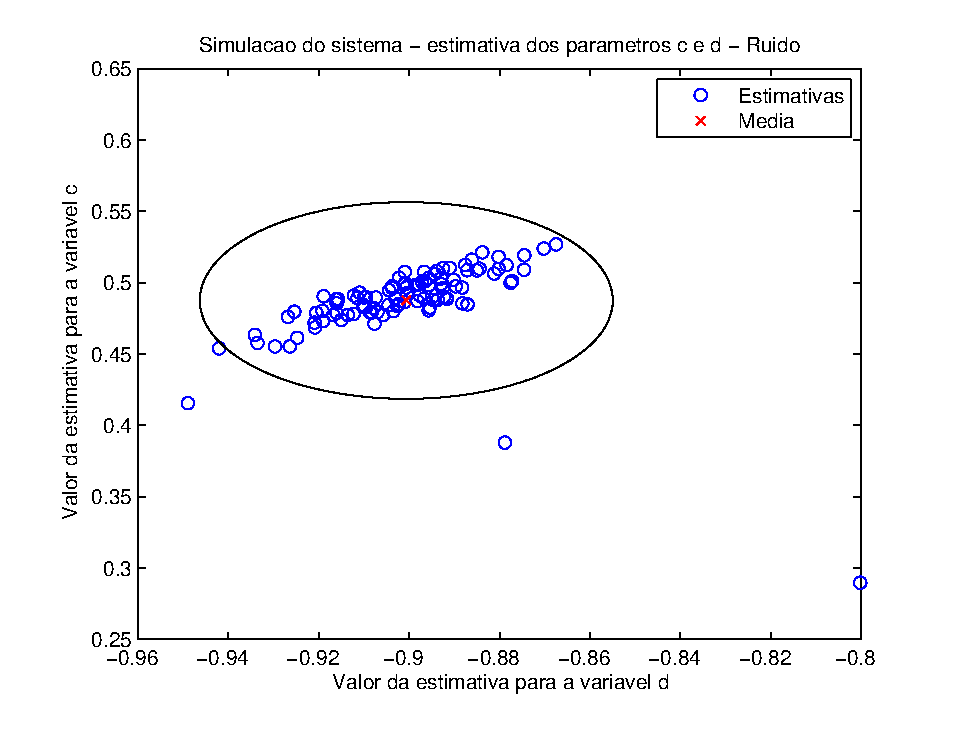
\includegraphics[width=0.98\columnwidth]{figures/gmq_cd.eps}
	\caption{Simulac�o do sistema para uma entrada aleat�ria e utilizando o modelo completo - 
		variaveis do ruido $H(q)$ $c$ e $d$.}
	\label{fig:gmq_cd}
\end{figure}

resultando em uma m�dia para as variaveis de 

ma =

    2.0000


mb =

    0.7748


mc =

   -0.9006


md =

    0.4875

	colocar isso em uma tabela.


